\section{Example}\label{sec:example}
\mkAgenda

\begin{frame}[fragile]{Example (C++)}
    \center
    \begin{minted}[linenos,breaklines=true]{C++}
void matmul_cpu(float *a, float *b, float *c, size_t m, size_t n, size_t p) {
  for(size_t i = 0; i < m; i++) {
    for(size_t j = 0; j < p; j++) {
      c[i * p + j] = 0;
      for(size_t k = 0; k < n; k++) {
        c[i * p + j] += a[i * n + k] * b[k * p + j];
      }
    }
  }
}
// ...
matmul_cpu(a, b, c, m, n, p);
    \end{minted}
\end{frame}

\begin{frame}[fragile]{Example (C++)}
    \center
    \begin{itemize}
        \item<1-> $\mathcal{O}(m \cdot n \cdot p)$ operations
        \item<2-> $m \cdot p$ independent (write different elements of \CUDA{c})
        \item<3-> Idea: launch $m \cdot p$ threads on GPU
    \end{itemize}
    \onslide<4->{
        \begin{block}{Synchronization}
            All threads should do independent work - synchronization is expensive!
        \end{block}
    }
\end{frame}

\subsection{Preparation}\label{subsec:preparation}
\begin{frame}[fragile]{Preparation}
    \center
    \begin{minted}[linenos,breaklines=true]{C++}
float *a, *b, *c;
size_t m, n, p;
// ... data is readied here ...
    \end{minted}
\end{frame}

\begin{frame}[fragile]{Preparation}
    \center
    Separate address spaces $\Rightarrow$ ready memory
    \begin{minted}[linenos,firstnumber=4,breaklines=true]{C++}
// create buffers on GPU ...
float *a_dev, *b_dev, *c_dev;
cudaMalloc(&a_dev, m * n * sizeof(float));
cudaMalloc(&b_dev, n * p * sizeof(float));
cudaMalloc(&c_dev, m * p * sizeof(float));
// ... and copy relevant data
cudaMemcpy(a_dev, a, m * n * sizeof(float), cudaMemcpyDefault);
cudaMemcpy(b_dev, b, n * p * sizeof(float), cudaMemcpyDefault);

// TODO: start GPU threads
    \end{minted}
\end{frame}

\begin{frame}[fragile]{Preparation}
    \center
    After GPU finishes, copy data back
    \begin{minted}[linenos,firstnumber=13,breaklines=true]{CUDA}
// TODO: start GPU threads

cudaMemcpy(c, c_dev, m * p * sizeof(float), cudaMemcpyDefault);
    \end{minted}
\end{frame}

\subsection{Kernel}\label{subsec:kernel}
\begin{frame}[fragile]{Kernel}
    \center
    \begin{itemize}
        \item<1-> Each function: execution space
        \item<2-> Three possible:
        \begin{itemize}
            \item<2-> \CUDA{__host__}: CPU only
            \item<2-> \CUDA{__device__}: GPU only
            \item<2-> \CUDA{__global__}: CPU to GPU entry
            \item<3-> Can combine \CUDA{__host__ __device__}
        \end{itemize}
    \end{itemize}
    \onslide<4->{
        \begin{block}{\CUDA{__global__}}
            Functions marked as \CUDA{__global__} should always be \CUDA{void}
        \end{block}
    }
\end{frame}

\begin{frame}[fragile]{Kernel}
    \center
    \begin{minted}[linenos,breaklines=true]{CUDA}
__global__ void matmul_gpu(float *a, float *b, float *c, size_t m, size_t n, size_t p) {
  size_t i = some_magic_trick();
  size_t j = some_other_magic_trick();
  c[i * p + j] = 0;
  for(size_t k = 0; k < n; k++) {
    c[i * p + j] += a[i * n + k] * b[k * p + j];
  }
}
    \end{minted}
    \begin{itemize}
        \item<2-> Notice keyword \CUDA{__global__}
        \item<3-> How to get \CUDA{i}, \CUDA{j}?
    \end{itemize}
\end{frame}

\begin{frame}[fragile]{Kernel}
    \center
    \begin{itemize}
        \item<1-> \CUDA{i}, \CUDA{j}? \textrightarrow use thread index
        \item<2-> Threads are launched in blocks of threads
        \item<3-> Sizes are defined in 3D
        \item<4-> Preferably launch in powers of 2
    \end{itemize}
    \onslide<3->{
        \centerline{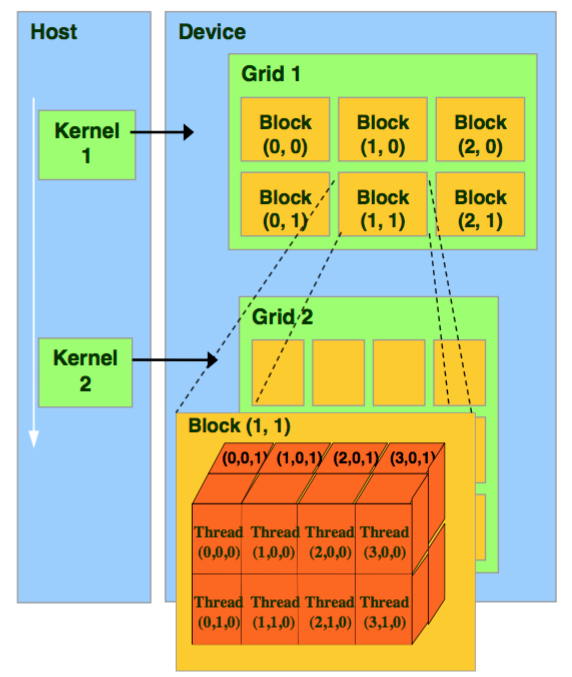
\includegraphics[width=0.33\textwidth]{./figures/thread-mapping}}
    }
\end{frame}

\begin{frame}[fragile]{Kernel}
    \center
    \begin{minted}[linenos,breaklines=true]{CUDA}
__global__ void matmul_gpu(float *a, float *b, float *c, size_t m, size_t n, size_t p) {
  size_t i = threadIdx.x + blockIdx.x * blockDim.x;
  size_t j = threadIdx.y + blockIdx.y * blockDim.y;
  if(i >= m || j >= p) return; // out of bounds
  c[i * p + j] = 0;
  for(size_t k = 0; k < n; k++) {
    c[i * p + j] += a[i * n + k] * b[k * p + j];
  }
}
    \end{minted}
\end{frame}

\subsection{Launch}\label{subsec:launch}
\begin{frame}[fragile]{Launch}
    \center
    \begin{itemize}
        \item<1-> Kernel launch using special syntax \CUDA{<<<>>>}
    \end{itemize}
    \onslide<2->{\centerline{\CUDA{matmul_gpu<<<blocks, threads>>>(args)}}}
    \begin{itemize}
        \item<3-> \CUDA{blocks} and \CUDA{threads} are \CUDA{dim3} values
        \item<4-> \CUDA{dim3(x)}, \CUDA{dim3(x, y)}, \CUDA{dim3(x, y, z)} are all valid
        \item<5-> Arguments are passed as normal
        \item<6-> Launch is asynchronous; wait for completion using \CUDA{cudaDeviceSynchronize()}
    \end{itemize}
\end{frame}

\begin{frame}[fragile]{Launch}
    \center
    \begin{minted}[linenos,firstnumber=10,breaklines=true]{CUDA}
// ...
cudaMemcpy(a_dev, a, m * n * sizeof(float), cudaMemcpyDefault);
cudaMemcpy(b_dev, b, n * p * sizeof(float), cudaMemcpyDefault);

auto blocks = dim3(m / 1024 + 1, p / 1024 + 1);
auto threads = dim3(1024, 1024);
matmul_gpu<<<blocks, threads>>>(a_dev, b_dev, c_dev, m, n, p);
cudaDeviceSynchronize(); // wait for GPU to finish

cudaMemcpy(c, c_dev, m * p * sizeof(float), cudaMemcpyDefault);
    \end{minted}
\end{frame}
